% !TEX root=/home/tavant/these/manuscript/src/manuscript.tex

\FloatBarrier
{\bf Conclusion: $\gamma = 1.35$ in presheath and $\partial{\gamma} / \partial \crover = 0 $}

\paragraph{Hypothesis H1: } Polytropic model until the wall and $\gamma = 1.35$ (might be explained by \cref{{fig-evdf_epsstar}}, and by the fact that we care only on the forward temperature, so not distorted by the secondary electrons).

\paragraph{Hypothesis H2: } From {\bf H1}, and with the 2-$\Te$ hypothesis, we have $\rate = \rate_{\rm Maxw}(\Tew)$, were $\Tew$ can be computed from $Teb$, $\gamma$ and $\dphi$.

\paragraph{Hypothesis H3: } Current equality at the wall : $\Gamma_i + \rate \Gamma_e = \Gamma_e$. This is not a surprising hypothesis.

\section{Sheath model with polytropic electron and SEE}

With {\bf H1, H2} and {\bf H3} we have, as developed in \cref{sec-fluidPIC} with \cref{eq-gi,eq-ge,eq-tew}:
\begin{equation}\label{eq-sheathsee}
  (1 - \rate_{\rm Maxw}(\Tew) )\left[ 1 +\frac{\gamma -1}{\gamma} \frac{ \dphi_0}{ \Te_0}  \right]^{\frac{1}{\gamma - 1}} \sqrt{1 - \frac{\gamma -1}{\gamma}\frac{\dphi_0}{\Te_0}} = \sqrt{\frac{4 \gamma \pi m_e}{m_i}}
\end{equation}
In contrast with \cref{eq-sheath}, now the sheath potential $\Delta \phi$ depends on $\rate$ with depends on $\Te$.
Hence, $\dphi$ is not fully normalized.

\begin{figure}[hbtp]
  \centering
  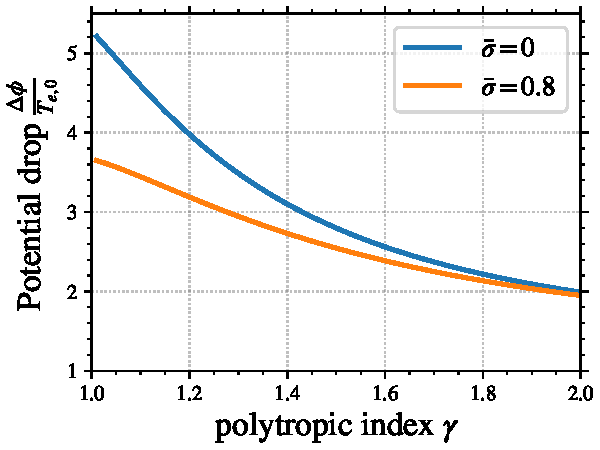
\includegraphics[width=\defaultwidth]{Sheath_drop_with_SEE.pdf}
  \caption{Potential drop $\dphi$ normilized by the bulk electron temperature $\Te_0$ as a function of the polytropic index $\gamma$ for a xenon plasma ($m_i = 131\,\dalton$). The emission rate $\rate$ is fixed for clarity.}
  \label{fig-dphi_see}
\end{figure}

\begin{figure}[hbtp]
  \centering
  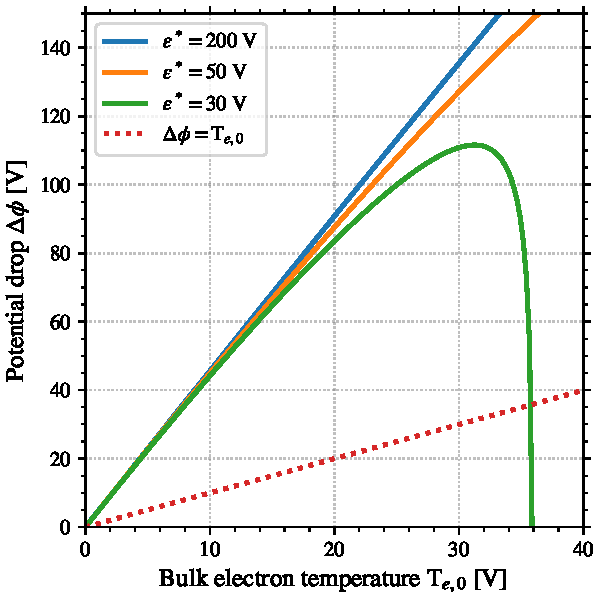
\includegraphics[width=\defaultwidth]{RSO_criteria_polytropic.pdf}
  \caption{ Plasma potential drop to the wall as a function of the electron temperature for different values of the cross-over energy $\crover$ using \cref{eq-sheathsee,eq-seemaxw}. The dashed line is $\dphi=\Te$. Similar to  \cref{fig-dphivsTe} but with polytropic electron of index $\gamma=1.35$}
  \label{fig-rso_crit_see}
\end{figure}

\FloatBarrier

\section{Comparison with PIC simulations} \label{subsec-picandmodel}

\begin{figure}[hbtp]
  \centering
  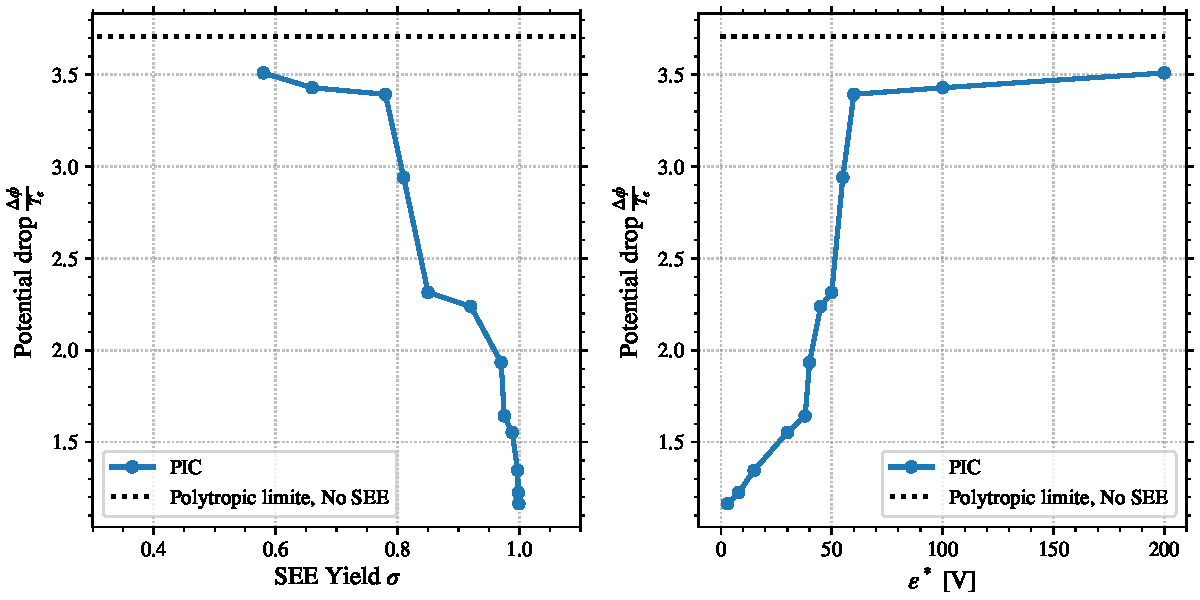
\includegraphics[width=\textwidth]{dphi_polytropic_noSEE}
  \caption{PIC simulation results (with SEE) compared to the polytropic limit without SEE.}
  \label{fig-polytropic_pic_noSEE}
\end{figure}

\begin{figure}[hbtp]
  \centering
  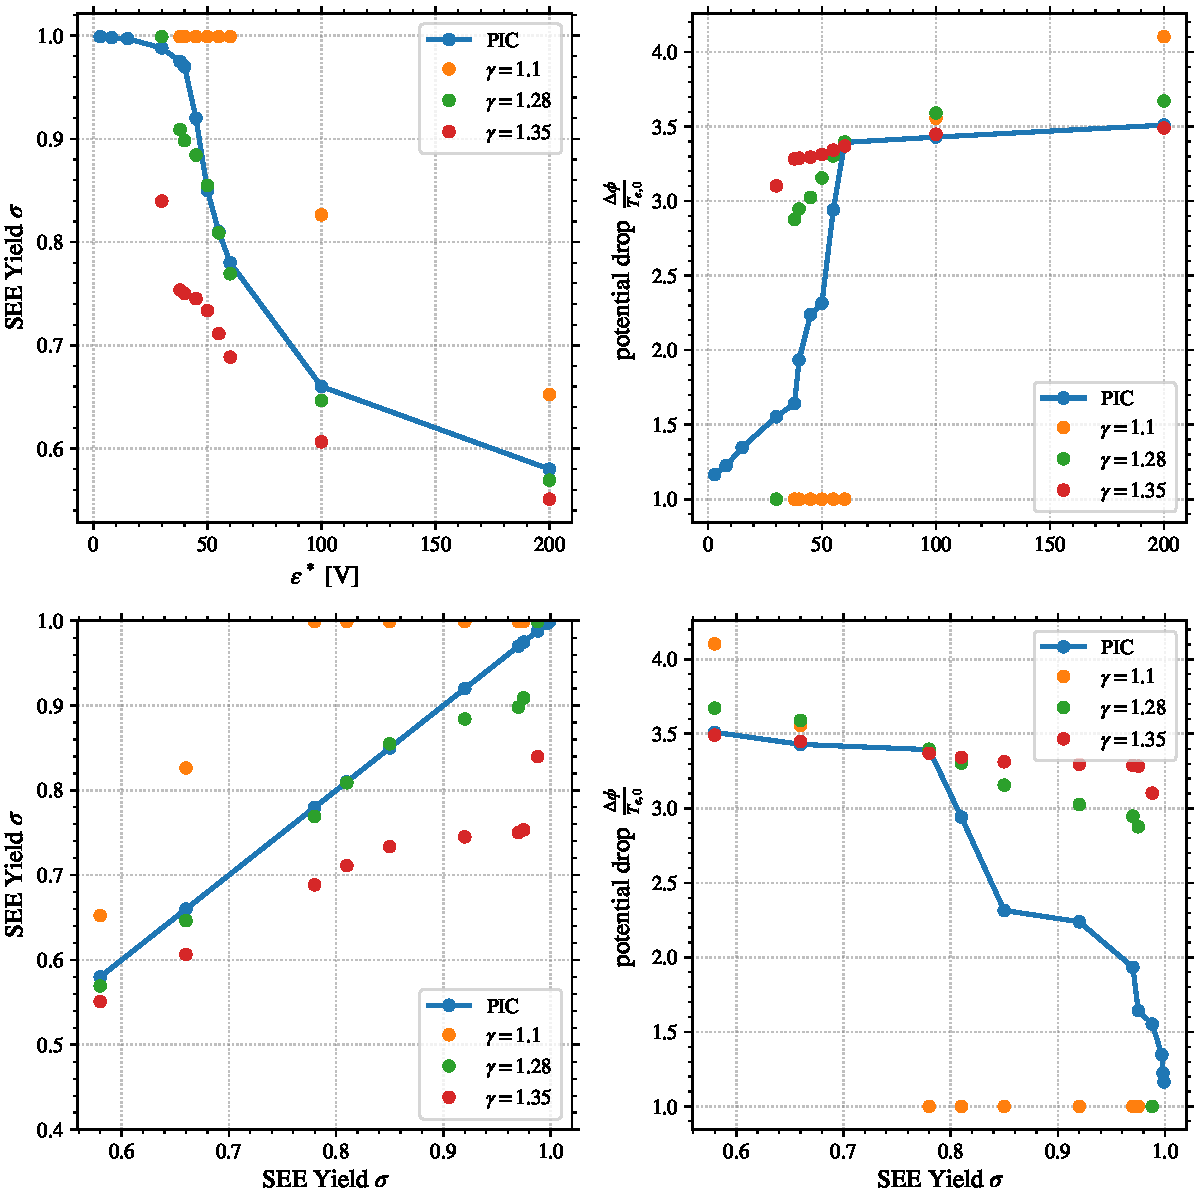
\includegraphics[width=\textwidth]{Summary_polytropic_SEE.pdf}
  \caption{Comparison of the PIC simulation results with the polytropic model with SEE.}
  \label{fig-polytropic_see_summary}
\end{figure}
